\section{Sélection d'un modèle}\label{chapter-ML-section-hyperparameters}
Deux types de modèle sont étudiés:
\begin{itemize}
\item des arbres de décision améliorés, introduits section~\ref{chapter-ML-section-XGB}, notés XGB;
\item des réseaux de neurones profonds, introduits section~\ref{chapter-ML-section-DNN}, notés DNN.
\end{itemize}
\par
Les hyperparamètres des XGBs sont:
\begin{itemize}
\item la profondeur maximale des arbres \MaxDepth;
\item la quantité d'échantillons minimale dans une branche \MinChildWeight;
\item le nombre d'arbres \Nestimators;
\item le gain minimal $\gamma$;
\item le taux d'apprentissage $\eta$;
\item la fonction de coût \Loss;
\item la liste des variables d'entrée.
\end{itemize}
\par
Les hyperparamètres des DNNs sont:
\begin{itemize}
\item le nombre de couches cachées $N_L$;
\item le nombre de neurones par couche cachée $N_N$;
\item la fonction d'activation des neurones (hormis celui de sortie);
\item la fonction de coût \Loss;
\item l'optimiseur;
\item le mode d'initiation des poids;
\item la liste des variables d'entrée.
\end{itemize}

no customized loss yet.

hard to get one single score to determine which model is the best: use mse, mae, mape, median diff, $\pm$ 1 or 2 $\sigma$ width ... low, medium, high and full mass regions as well.


\subsection{Variables d'entrée}

Model inputs : DNN not that sensible but XGB is better when having all of them, then use all inputs (give list) and not a subset of them.

\todo{use plots with ref when relevant}

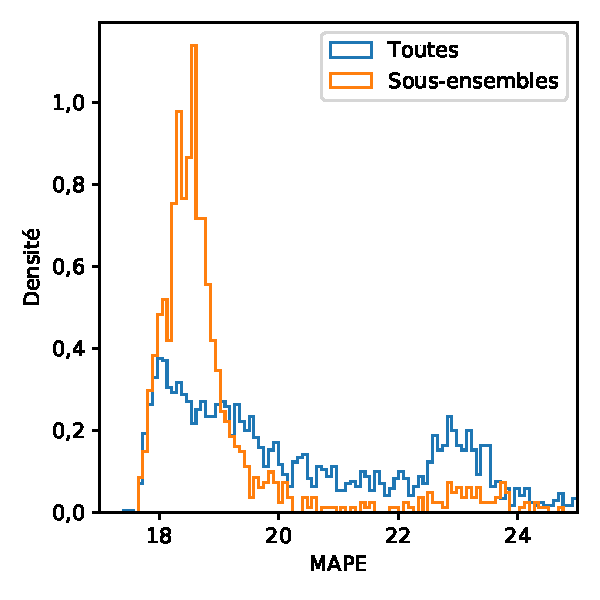
\includegraphics[width=.45\textwidth]{\PhDthesisdir/plots_and_images/my_plots/ML/from_ML_plots/global_comparisons/DNN_inputs-full_mape.pdf}
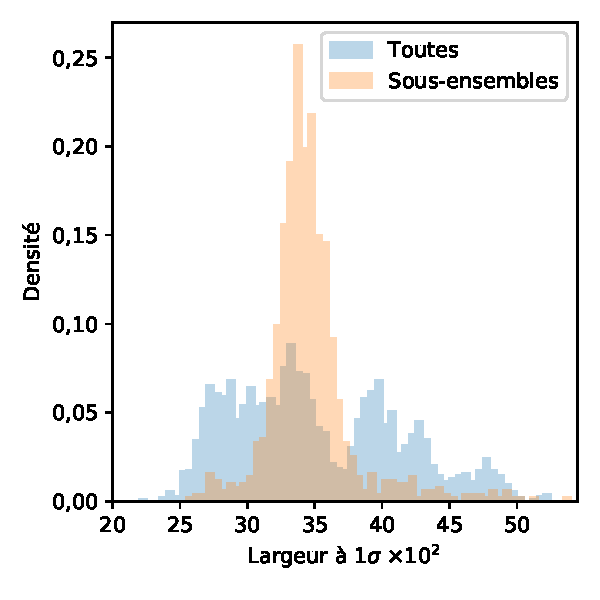
\includegraphics[width=.45\textwidth]{\PhDthesisdir/plots_and_images/my_plots/ML/from_ML_plots/global_comparisons/DNN_inputs-full_1sig_width.pdf}

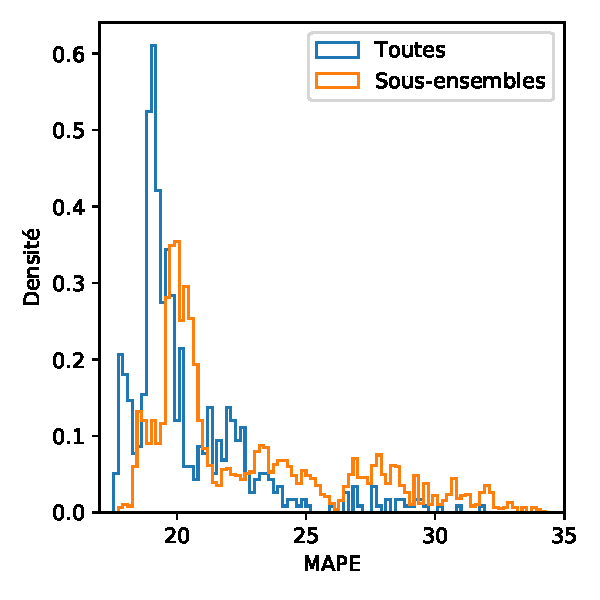
\includegraphics[width=.45\textwidth]{\PhDthesisdir/plots_and_images/my_plots/ML/from_ML_plots/global_comparisons/XGB_inputs-full_mape.pdf}
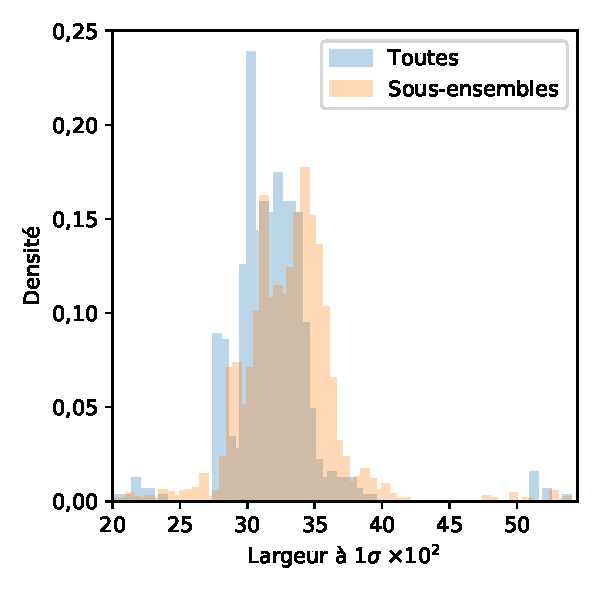
\includegraphics[width=.45\textwidth]{\PhDthesisdir/plots_and_images/my_plots/ML/from_ML_plots/global_comparisons/XGB_inputs-full_1sig_width.pdf}


\subsection{Type de modèle}

DNN vs XGB: use DNN!


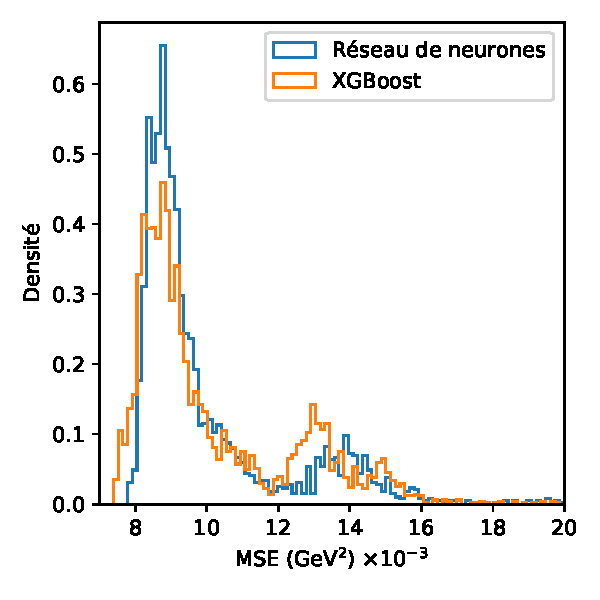
\includegraphics[width=.45\textwidth]{\PhDthesisdir/plots_and_images/my_plots/ML/from_ML_plots/global_comparisons/DNN_vs_XGB-full_mse.pdf}
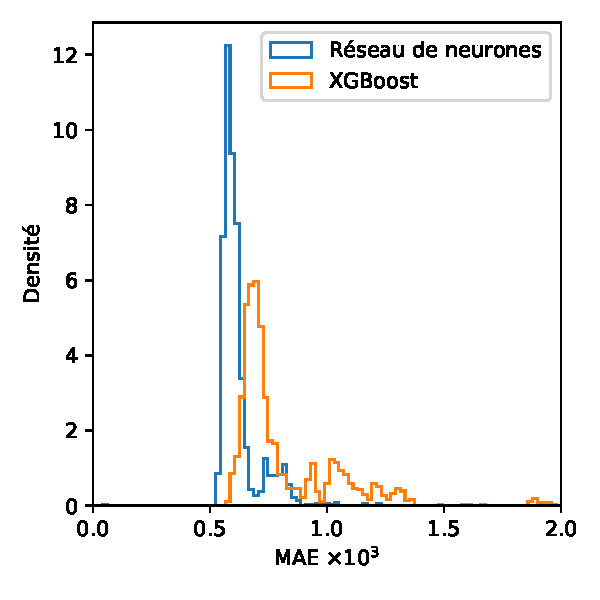
\includegraphics[width=.45\textwidth]{\PhDthesisdir/plots_and_images/my_plots/ML/from_ML_plots/global_comparisons/DNN_vs_XGB-full_mae.pdf}

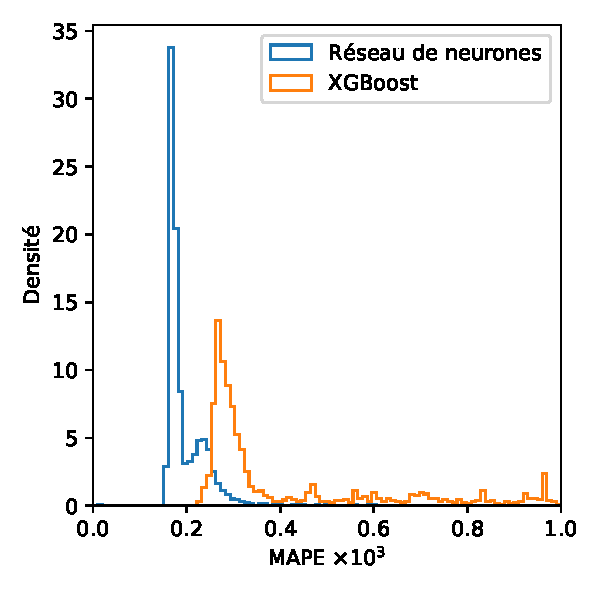
\includegraphics[width=.45\textwidth]{\PhDthesisdir/plots_and_images/my_plots/ML/from_ML_plots/global_comparisons/DNN_vs_XGB-full_mape.pdf}

\subsection{Fonction de coût}

loss: when using a given loss, the corresponding models are of course better when using the loss as score.

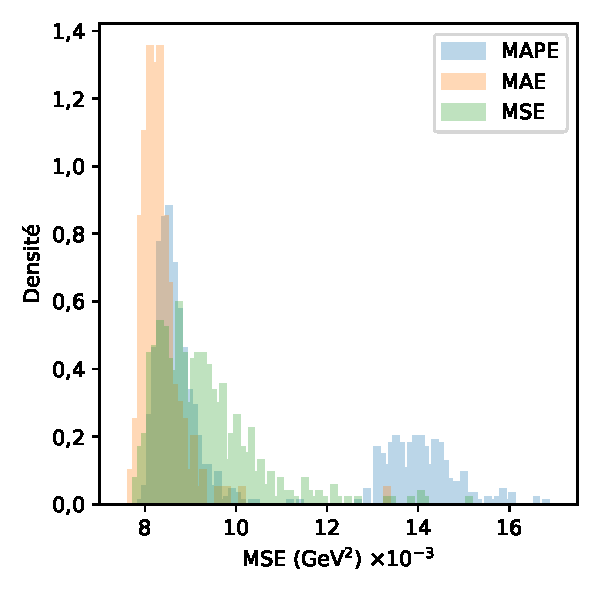
\includegraphics[width=.45\textwidth]{\PhDthesisdir/plots_and_images/my_plots/ML/from_ML_plots/global_comparisons/DNN_loss-full_mse.pdf}
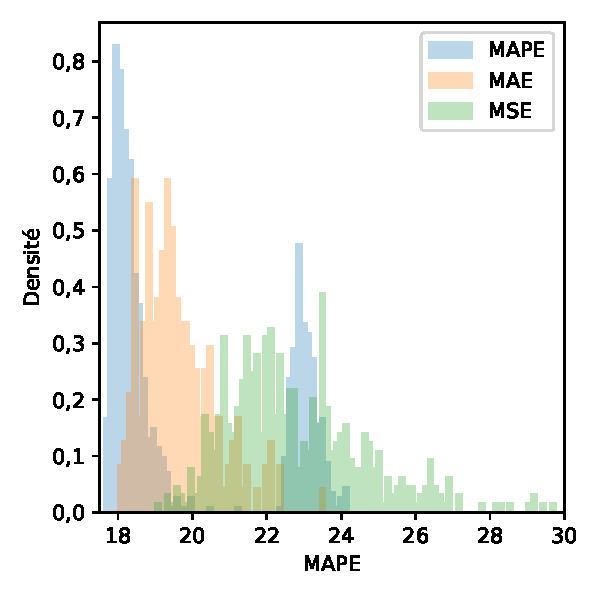
\includegraphics[width=.45\textwidth]{\PhDthesisdir/plots_and_images/my_plots/ML/from_ML_plots/global_comparisons/DNN_loss-full_mape.pdf}



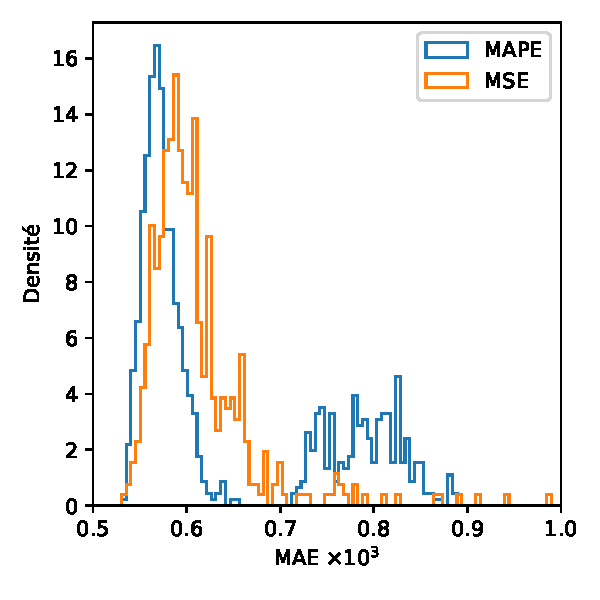
\includegraphics[width=.45\textwidth]{\PhDthesisdir/plots_and_images/my_plots/ML/from_ML_plots/global_comparisons/DNN_loss-full_mae.pdf}


use mape loss, gives the better results

\subsection{Initialisation des poids et optimisation}

optimizer: Adam

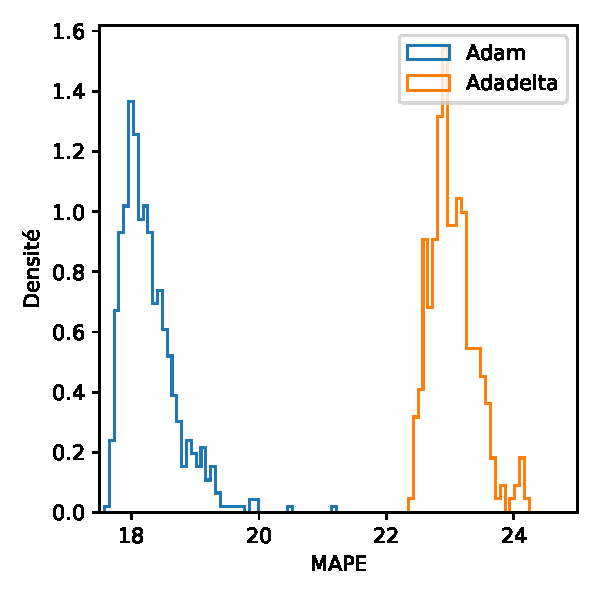
\includegraphics[width=.45\textwidth]{\PhDthesisdir/plots_and_images/my_plots/ML/from_ML_plots/global_comparisons/DNN_optimizer-full_mape.pdf}

w init mode Glorot Uniform

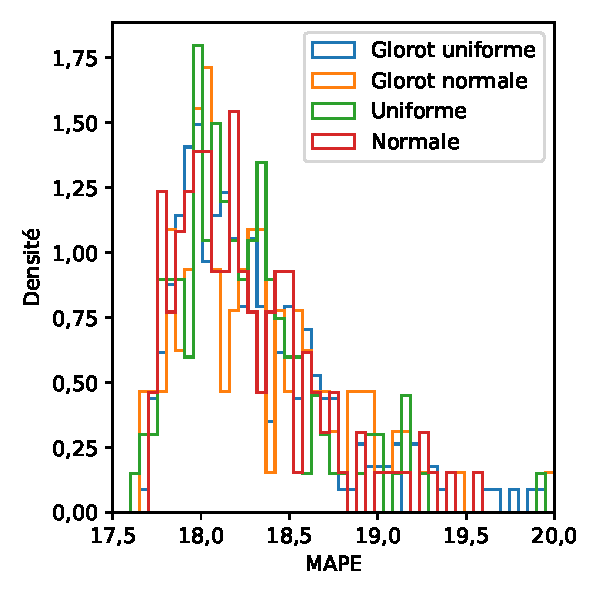
\includegraphics[width=.45\textwidth]{\PhDthesisdir/plots_and_images/my_plots/ML/from_ML_plots/global_comparisons/DNN_w_init_mode-full_mape.pdf}

\subsection{Structure}
which structure ?

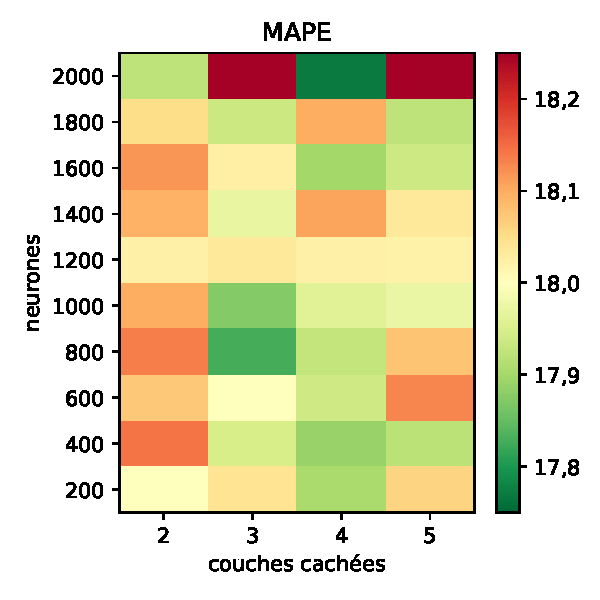
\includegraphics[width=.45\textwidth]{\PhDthesisdir/plots_and_images/my_plots/ML/from_ML_plots/global_comparisons/DNN_structures_reduced-full_mape.pdf}
%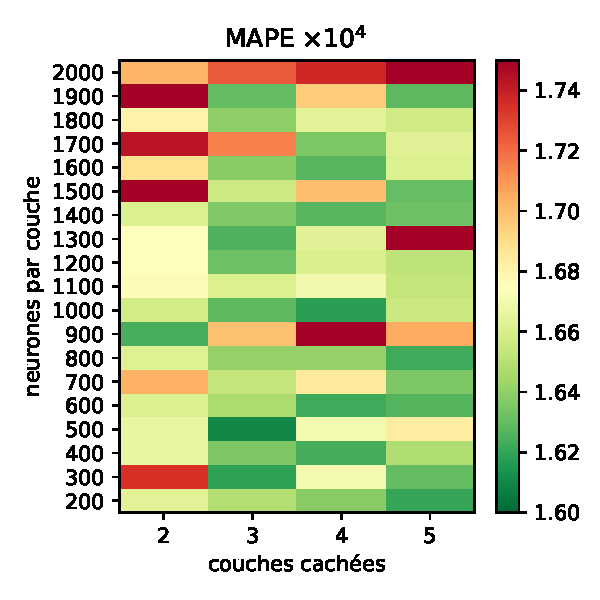
\includegraphics[width=.45\textwidth]{\PhDthesisdir/plots_and_images/my_plots/ML/from_ML_plots/global_comparisons/DNN_structures_all-full_mape.pdf}

several possibilities, but the loss mass region contains the Z boson and is important

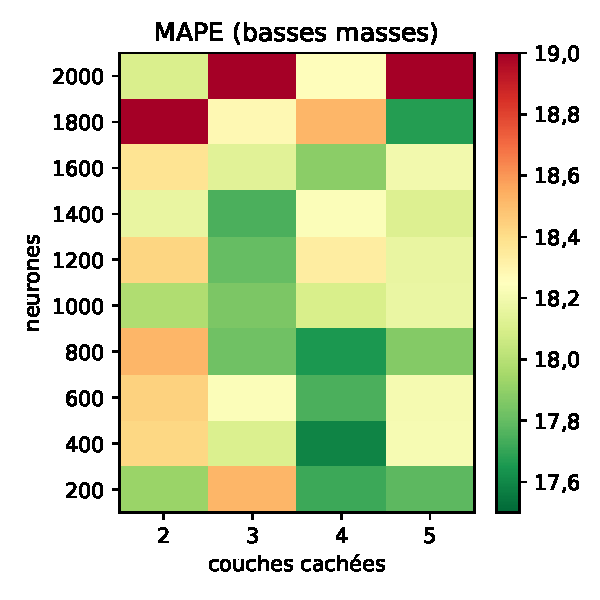
\includegraphics[width=.45\textwidth]{\PhDthesisdir/plots_and_images/my_plots/ML/from_ML_plots/global_comparisons/DNN_structures_reduced-low_mape.pdf}
%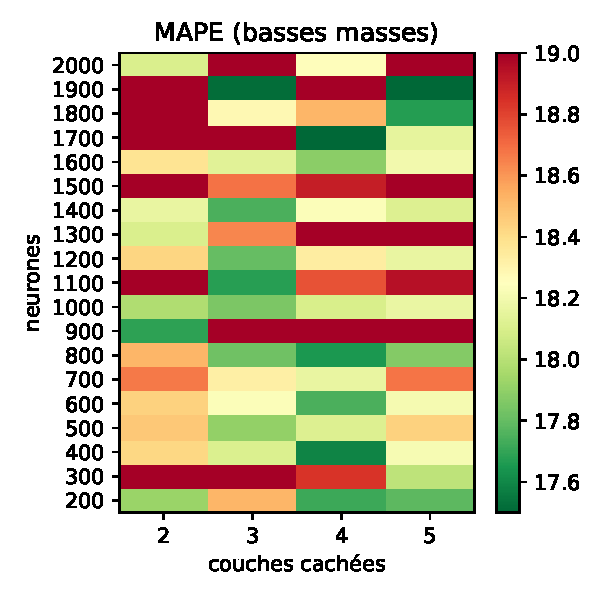
\includegraphics[width=.45\textwidth]{\PhDthesisdir/plots_and_images/my_plots/ML/from_ML_plots/global_comparisons/DNN_structures_all-low_mape.pdf}

2x900 and 5x600 seem to be the best options, check the low mass resolution

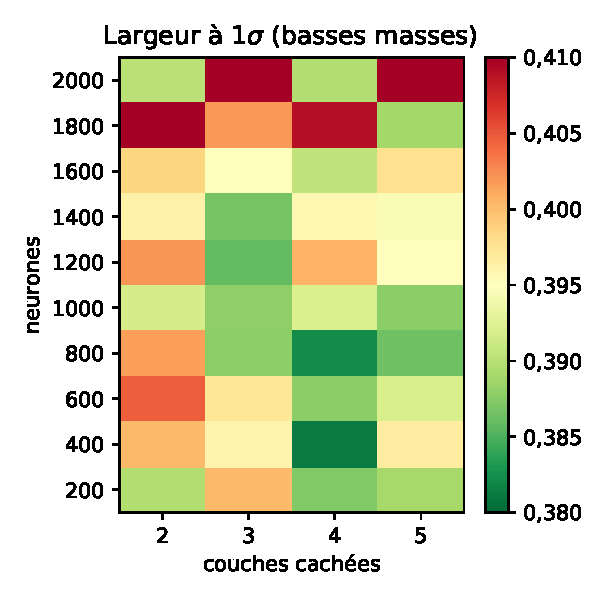
\includegraphics[width=.45\textwidth]{\PhDthesisdir/plots_and_images/my_plots/ML/from_ML_plots/global_comparisons/DNN_structures_reduced-low_1sig_width.pdf}
%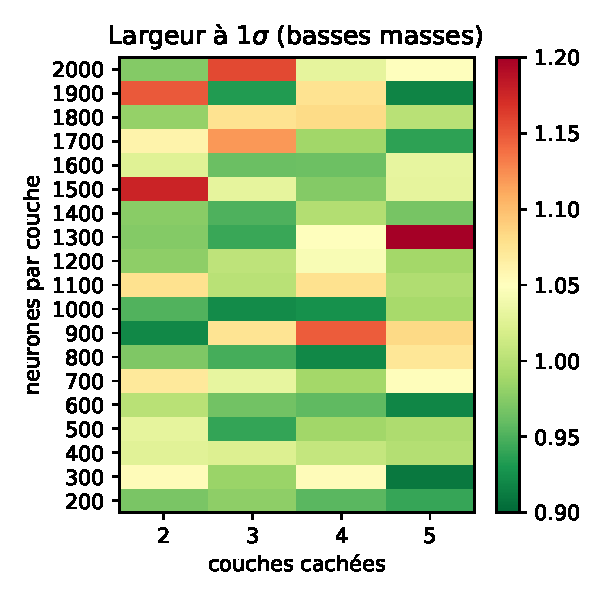
\includegraphics[width=.45\textwidth]{\PhDthesisdir/plots_and_images/my_plots/ML/from_ML_plots/global_comparisons/DNN_structures_all-low_1sig_width.pdf}

5x600 seems good, check the low mass \textbf{calibrated} resolution

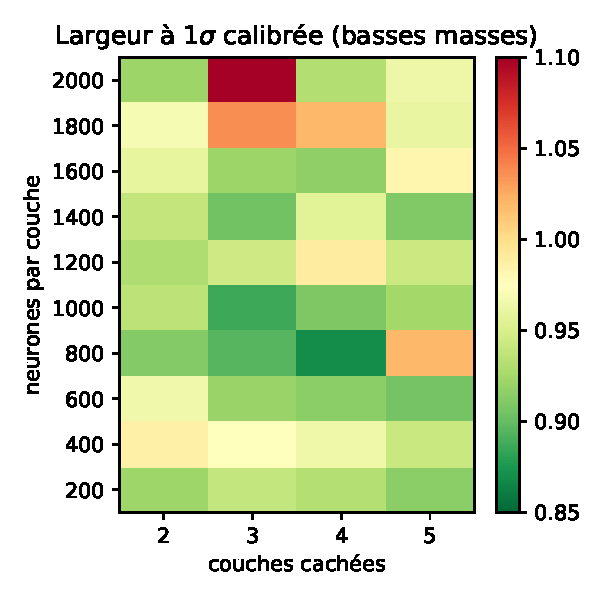
\includegraphics[width=.45\textwidth]{\PhDthesisdir/plots_and_images/my_plots/ML/from_ML_plots/global_comparisons/DNN_structures_reduced-low_1sig_calibr_width.pdf}
%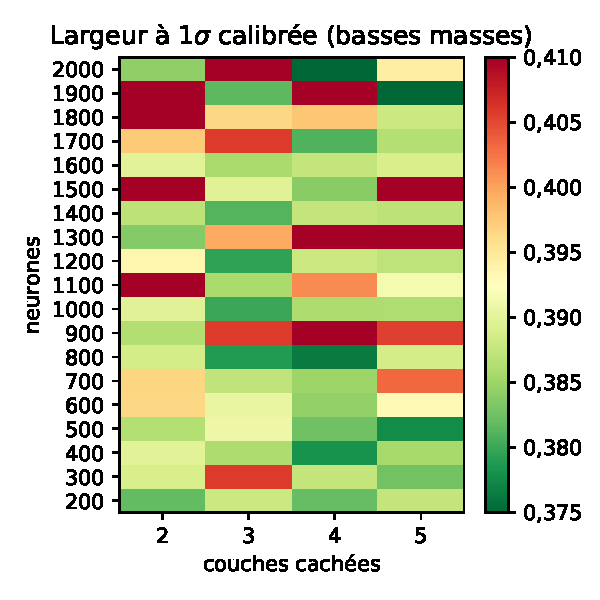
\includegraphics[width=.45\textwidth]{\PhDthesisdir/plots_and_images/my_plots/ML/from_ML_plots/global_comparisons/DNN_structures_all-low_1sig_calibr_width.pdf}

and in the medium mass region we have

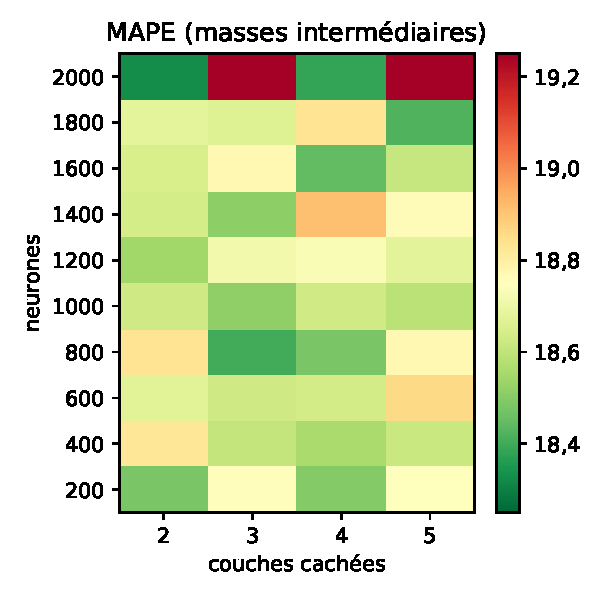
\includegraphics[width=.45\textwidth]{\PhDthesisdir/plots_and_images/my_plots/ML/from_ML_plots/global_comparisons/DNN_structures_reduced-medium_mape.pdf}
%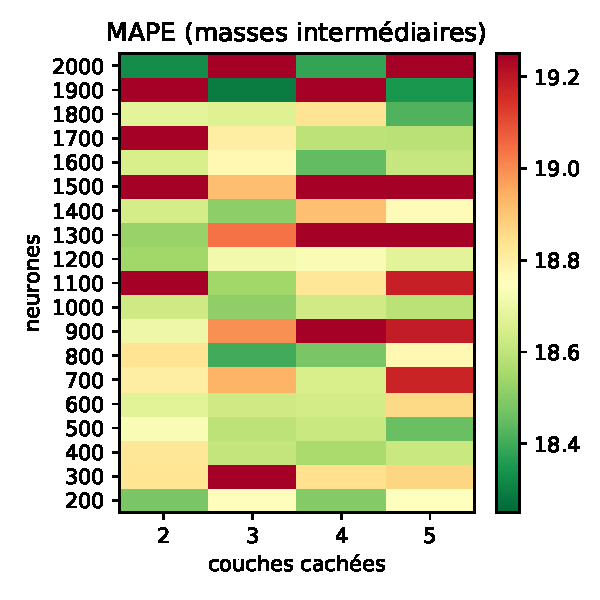
\includegraphics[width=.45\textwidth]{\PhDthesisdir/plots_and_images/my_plots/ML/from_ML_plots/global_comparisons/DNN_structures_all-medium_mape.pdf}

3x1000 is the best compromise we found

\subsection{Fonction d'activation}

activation = softplus

